\documentclass[11pt,letterpaper]{article}

\usepackage{fontspec}
\setmainfont{Times New Roman}
\usepackage{polyglossia}
\setdefaultlanguage{spanish}

\usepackage[margin=2.3cm]{geometry}
\usepackage{graphicx}
\usepackage{booktabs}
\usepackage{array}
\usepackage{amsmath}
\usepackage{unicode-math}
\setmathfont{TeX Gyre Termes Math}
\usepackage{caption}
\usepackage{float}
\usepackage[table]{xcolor}
\usepackage{fancyhdr}
\usepackage[hidelinks]{hyperref}
\usepackage{enumitem}
\usepackage{tabularx}
\usepackage{tikz}
\usetikzlibrary{positioning,arrows.meta,shapes.geometric}

\linespread{1.12}
\setlength{\parskip}{0.5em}
\setlength{\parindent}{0pt}
\captionsetup{font=small,labelfont=bf,skip=4pt}
\setlist{itemsep=0.15em,topsep=0.3em}
\newcolumntype{Y}{>{\raggedright\arraybackslash}X}

\pagestyle{fancy}
\fancyhf{}
\fancyhead[L]{\small CC3084 --- Laboratorio 11: MLOps del observatorio}
\fancyhead[R]{\small\thepage}
\renewcommand{\headrulewidth}{0.4pt}

\newcommand{\run}[1]{\texttt{#1}}

\begin{document}
\sloppy

\begin{titlepage}
\centering
\vspace*{0.2cm}

\includegraphics[width=3.6cm]{../../Informe/logouvg.png}

\vspace{0.5cm}
{\large Universidad del Valle de Guatemala}\\[0.2em]
{\large Facultad de Ingeniería}\\[0.2em]
{\large Departamento de Ciencias de la Computación}\\[0.2em]
{\large CC3084 --- Data Science --- Semestre II, 2026}

\vspace{1.0cm}
\rule{\textwidth}{1.2pt}
\vspace{0.6cm}

{\Huge\bfseries Laboratorio 11}\\[0.6em]
{\LARGE MLOps aplicado al Observatorio de Inteligencia Turística}\\[0.9em]
{\large Informe técnico: flujo reproducible, validación temporal,}\\[0.2em]
{\large regla de aceptación, fallo y recuperación}

\vspace{0.6cm}
\rule{\textwidth}{1.2pt}

\vspace{1.2cm}
{\large\bfseries Integrantes}\\[0.8em]
{\large Rodrigo Ajmac --- 22279}\\[0.3em]
{\large Andrés Mazariegos --- 21749}\\[0.3em]
{\large June Herrera --- 231038}\\[0.3em]
{\large Sebastián García --- 22291}

\vfill
{\large Guatemala, 1 de noviembre de 2026}\\[0.3em]
{\small Código: rama \texttt{Lab11}, carpeta \texttt{lab11/} del repositorio del grupo}
\end{titlepage}

\tableofcontents
\newpage

%==========================================================
\section{Alcance del flujo}

El flujo actualiza de forma controlada la estimación mensual de visitantes que ingresan a Guatemala. Además deja registro de qué datos, código y configuración produjeron cada cifra que consulta un directivo en el tablero del Laboratorio~10.

\begin{table}[H]
\centering\small
\caption{Definición del alcance.}
\begin{tabularx}{\textwidth}{@{}p{3.6cm}Y@{}}
\toprule
Destino & Guatemala (país completo). \\
Variable & Visitantes no residentes: suma de \texttt{Viajero} excluyendo las filas con \texttt{País = Guatemala}. \\
Unidad y agregación & Viajeros por mes calendario. Es un conteo de registros de ingreso, no de personas únicas. \\
Fuente & \texttt{Base\_Migracion\_2009-2026jun.xlsx}, hoja mensual \texttt{Datos} (161\,036 filas). Clave: \texttt{Año}, \texttt{Mes cod}, \texttt{Vía}, \texttt{Frontera}, \texttt{País}, \texttt{Región}, \texttt{Región dos}, \texttt{Regiones OMT}, \texttt{MCEO}, \texttt{Agrupación Residencia}, \texttt{Tipo de Viajero}. Valor: \texttt{Viajero}. \\
Cobertura exigida & Enero 2009 -- junio 2026 (210 meses). \\
Período de ajuste & Enero 2022 -- junio 2026. \\
Evaluación & Orígenes junio y diciembre de 2025, seis meses ocultos en cada uno: julio 2025 -- junio 2026. \\
Estimaciones & Julio -- diciembre 2026. \\
Procedimiento & Versión 2.0, ingenuo estacional: $\hat y_t = y_{t-12}$. \\
Factor de reparto & 1: la variable sale directamente de los conteos mensuales del país, sin repartirse a otra granularidad. \\
Salida del tablero & \texttt{publicado/vigente.json} $\rightarrow$ \texttt{versiones/<run\_id>/estimaciones.csv}. \\
\bottomrule
\end{tabularx}
\end{table}

\textbf{Cambio respecto del avance.} El avance estimaba el total de viajeros. Desde enero de 2023 la fuente dejó de registrar a los guatemaltecos que regresan, y el total cae entre 150 y 200 mil viajeros por mes solo por ese cambio de medición. Ajustar un modelo sobre ese corte sesgaría la estimación. Por eso la variable excluye a los residentes en todo el período, igual que la opción «no residentes» del tablero. La regla metodológica (sección~\ref{sec:controles}) impide volver a mezclar meses con y sin esa cobertura.

\textbf{Meses sin la variable.} Entre abril y agosto de 2020 (cierre de fronteras) la fuente solo registra residentes. Esos meses quedan ausentes, no en cero. Como están antes del período de ajuste, solo producen una advertencia.

%==========================================================
\section{Diagrama del flujo}

\begin{figure}[H]
\centering
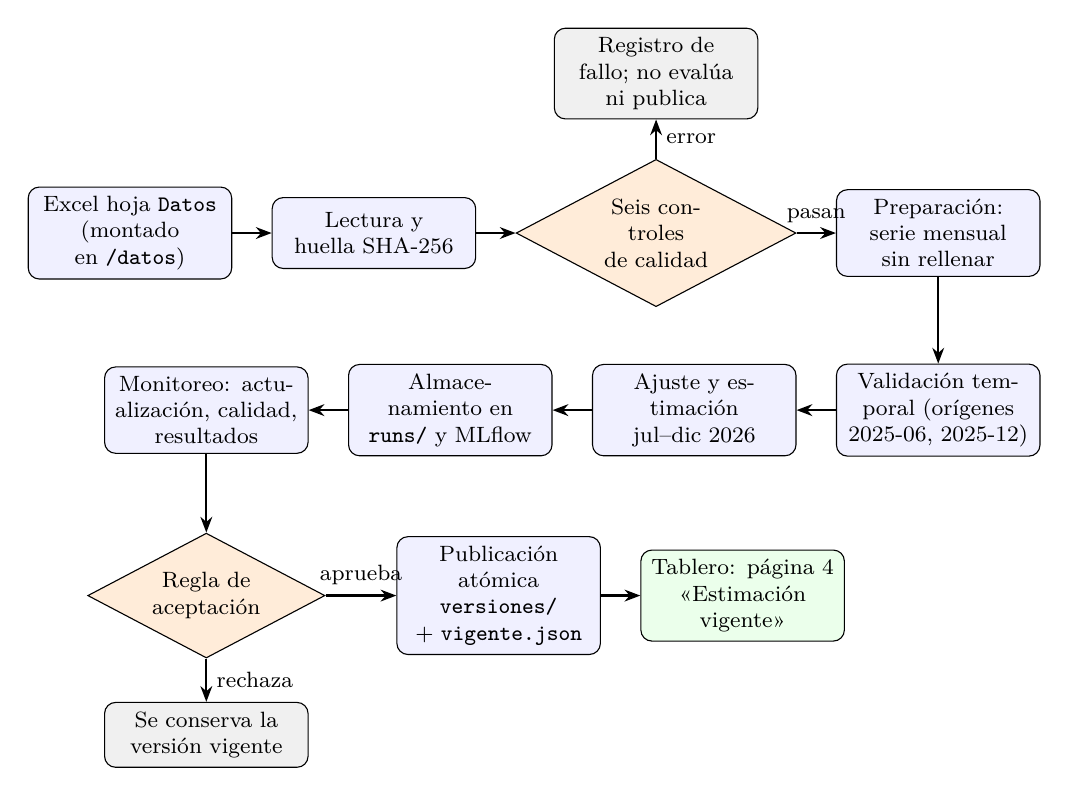
\begin{tikzpicture}[node distance=0.55cm and 0.5cm, font=\footnotesize,
  caja/.style={draw, rounded corners, fill=blue!6, align=center, minimum height=0.9cm, text width=2.35cm},
  dec/.style={draw, diamond, aspect=1.9, fill=orange!15, align=center, inner sep=1pt, text width=1.7cm},
  fin/.style={draw, rounded corners, fill=gray!12, align=center, text width=2.35cm, minimum height=0.8cm},
  flecha/.style={-{Stealth[length=2mm]}, thick}]
\node[caja] (a) {Excel hoja \texttt{Datos}\\(montado en \texttt{/datos})};
\node[caja, right=of a] (b) {Lectura y huella SHA-256};
\node[dec, right=of b] (c) {Seis controles\\de calidad};
\node[caja, right=of c] (d) {Preparación: serie mensual sin rellenar};
\node[caja, below=1.1cm of d] (e) {Validación temporal (orígenes 2025-06, 2025-12)};
\node[caja, left=of e] (f) {Ajuste y estimación jul--dic 2026};
\node[caja, left=of f] (g) {Almacenamiento en \texttt{runs/} y MLflow};
\node[caja, left=of g] (h) {Monitoreo: actualización, calidad, resultados};
\node[dec, below=1.0cm of h] (i) {Regla de\\aceptación};
\node[caja, right=0.9cm of i] (j) {Publicación atómica \texttt{versiones/} + \texttt{vigente.json}};
\node[caja, right=of j, fill=green!8] (k) {Tablero: página 4 «Estimación vigente»};
\node[fin, above=0.5cm of c] (x) {Registro de fallo; no evalúa ni publica};
\node[fin, below=0.55cm of i] (y) {Se conserva la versión vigente};
\draw[flecha] (a) -- (b);
\draw[flecha] (b) -- (c);
\draw[flecha] (c) -- node[above]{pasan} (d);
\draw[flecha] (c) -- node[right]{error} (x);
\draw[flecha] (d) -- (e);
\draw[flecha] (e) -- (f);
\draw[flecha] (f) -- (g);
\draw[flecha] (g) -- (h);
\draw[flecha] (h) -- (i);
\draw[flecha] (i) -- node[above]{aprueba} (j);
\draw[flecha] (i) -- node[right]{rechaza} (y);
\draw[flecha] (j) -- (k);
\end{tikzpicture}
\caption{Flujo desde la lectura de la fuente hasta la consulta del tablero. Los datos se validan en los controles de calidad, el procedimiento se evalúa en la validación temporal y la publicación se autoriza en la regla de aceptación.}
\end{figure}

%==========================================================
\section{Pipeline reproducible y configuración}

Todo el flujo se ejecuta con un solo comando:

\begin{center}\texttt{docker compose run --rm pipeline}\end{center}

\texttt{lab11/pipeline.py} recorre las etapas de lectura, validación, preparación, evaluación, ajuste, estimación, almacenamiento, monitoreo, aceptación y publicación. Nadie modifica archivos intermedios a mano: cada ejecución escribe en su propia carpeta \texttt{runs/<run\_id>/} y no depende de una sesión previa. El tablero solo lee la versión publicada, así que cambiar un filtro nunca vuelve a ajustar el modelo.

\texttt{config.json} reúne rutas, períodos, método, parámetros del modelo, semilla (42), umbrales de aceptación, umbrales de monitoreo y la tolerancia de reproducibilidad. Las dependencias están fijadas en \texttt{requirements.txt} (pandas 2.2.3, numpy 2.2.3, openpyxl 3.1.5, statsmodels 0.14.4, MLflow 2.22.0, SQLAlchemy 2.0.41, Streamlit 1.66.0, Plotly 5.24.1) y la imagen parte de \texttt{python:3.12.10-slim}. Cada ejecución registra en MLflow las versiones que realmente usó. La fórmula del procedimiento y sus valores base se guardan como \texttt{modelo/parametros.json}. En Holt-Winters también se guardan los parámetros de suavizado y el modelo serializado.

Códigos de salida: 0 publicada, 3 rechazada por la regla, 1 fallida.

%==========================================================
\section{Controles automáticos de calidad}\label{sec:controles}

\begin{table}[H]
\centering\footnotesize
\caption{Seis controles. Un \emph{error} detiene el flujo antes de evaluar y no toca la versión publicada.}
\begin{tabularx}{\textwidth}{@{}p{2.3cm}YYY@{}}
\toprule
Control & Qué verifica & Advertencia & Detiene \\
\midrule
Columnas y tipos & Las 12 columnas indispensables; \texttt{Año}, \texttt{Mes cod} y \texttt{Viajero} numéricas; categorías de texto & --- & Columna ausente o tipo incompatible \\
Fechas y cobertura & Año y mes válidos; registros en los 210 meses; variable presente en todo el período de ajuste & Meses sin la variable antes del ajuste; meses fuera de la cobertura & Fecha inválida, mes sin registros o mes del ajuste sin la variable \\
Unicidad & Una fila por combinación de las 11 dimensiones y mes & --- & Clave duplicada \\
Valores faltantes & Una categoría sin fila equivale a cero viajeros en ella (permitido); no hay nulos en campos indispensables & Faltantes en \texttt{Mes} $>$ 5\,\% & Nulo indispensable \\
Valores y denominadores & \texttt{Viajero} finito y $\ge 0$; denominador del WAPE $\neq 0$ & Mes evaluado igual a cero (se excluye del MAPE) & Negativo, no finito o denominador cero \\
Regla metodológica & La serie viene de la hoja mensual (\texttt{Año}, \texttt{Mes cod}), no de fechas diarias; no mezcla meses con y sin cobertura de residentes & Los residentes reaparecen después de 2023 & Otra hoja, columna diaria o mezcla de coberturas \\
\bottomrule
\end{tabularx}
\end{table}

Con la fuente oficial pasan los seis controles: 0 duplicados, 0 faltantes indispensables y 0 conteos inválidos. La única advertencia corresponde a los meses de 2020 sin no residentes. Dieciocho pruebas con datos sintéticos (\texttt{tests/test\_pipeline.py}) comprueban que cada control detiene el flujo o advierte cuando corresponde. También verifican que un mes ausente no se convierte en cero.

%==========================================================
\section{Registro y trazabilidad en MLflow}

El experimento \texttt{observatorio-guatemala-no-residentes} vive en un servidor MLflow con base SQLite y artefactos servidos por el propio servidor (\texttt{lab11/mlflow\_data}, montado como volumen). Cada ejecución registra:

\begin{itemize}
\item Identificador y fecha; etiqueta \texttt{git\_commit} y \texttt{codigo\_modificado\_sin\_commit}.
\item \texttt{fuente\_archivo}, \texttt{fuente\_sha256} y \texttt{config\_sha256}; períodos de ajuste y evaluación.
\item Parámetros, métricas (\texttt{proc\_*}, \texttt{ref\_*}, \texttt{ctx\_*}), resultado de cada control (\texttt{control\_*\_ok}) y del monitoreo.
\item Artefactos: configuración, reporte de calidad, serie preparada, evaluación mes a mes, estimaciones, monitoreo, decisión de aceptación, parámetros del procedimiento y registro de la ejecución.
\end{itemize}

\begin{table}[H]
\centering\footnotesize
\caption{Ejecuciones registradas (exportadas con \texttt{consultar\_mlflow.py} a \texttt{evidencia/ejecuciones\_mlflow.csv}). Hora UTC del 1 de noviembre de 2026.}
\begin{tabular}{@{}lllllll@{}}
\toprule
Run & Hora & Estado & Versión & Commit & Fuente & WAPE \\
\midrule
\run{f169bf4b} & 18:49 & rechazada & 1.0 & \run{ac08bbe} & oficial & 8,4\,\% \\
\run{bb4cc75c} & 18:49 & rechazada & 1.0$^{a}$ & \run{78bf214} & oficial & 8,4\,\% \\
\run{0a6b9210} & 18:50 & rechazada & 1.0$^{a}$ & \run{78bf214} & oficial & 8,4\,\% \\
\run{eb8c3bf0} & 18:51 & publicada & 2.0 & \run{7f2f531} & oficial & 4,1\,\% \\
\run{eef1c71e} & 18:52 & publicada & 2.0 & \run{7f2f531} & oficial & 4,1\,\% \\
\run{9b08a79e} & 18:54 & \textbf{FAILED} (unicidad) & 2.0 & \run{7f2f531} & clave duplicada & --- \\
\run{a15ea0ac} & 18:55 & \textbf{FAILED} (columnas) & 2.0 & \run{7f2f531} & columna ausente & --- \\
\run{3141c3ed} & 18:56 & rechazada & 2.0 & \run{7f2f531} & variación elevada & 20,6\,\% \\
\run{50752886} & 18:57 & publicada & 2.0 & \run{7f2f531} & copia corregida & 4,1\,\% \\
\run{c5332d00} & 21:01 & publicada & 2.0 & \run{25d8ead} & oficial & 4,1\,\% \\
\run{e528864e} & 21:01 & publicada (vigente) & 2.0 & \run{25d8ead} & oficial & 4,1\,\% \\
\bottomrule
\end{tabular}

\raggedright\footnotesize $^{a}$ La imagen Docker conservaba la configuración vieja. MLflow lo dejó registrado con \texttt{codigo\_modificado\_sin\_commit=true}. A partir de ahí el servicio monta \texttt{lab11/} para usar siempre el commit actual.
\end{table}

Las dos ejecuciones fallidas se detuvieron en la etapa de validación. Tienen estado \texttt{FAILED}, etiquetas \texttt{etapa\_fallida} y \texttt{error}, y no tienen métricas de evaluación, porque no llegaron a esa etapa.

\textbf{Reproducibilidad.} Si la versión vigente se generó con la misma huella de fuente y de configuración, el pipeline compara las estimaciones. Hubo tres comparaciones: \run{eb8c3bf0}$\rightarrow$\run{eef1c71e}, \run{c5332d00}$\rightarrow$\run{e528864e} y una ejecución desde una copia limpia del repositorio (\run{cfd88935}, \texttt{evidencia/copia\_limpia/}). En las tres la diferencia relativa máxima fue $1{,}1\times10^{-16}$: es redondeo de punto flotante, y la tolerancia configurada es $10^{-6}$. Al revisar la copia limpia apareció un problema: la huella de \texttt{config.json} cambiaba con los finales de línea LF/CRLF. Se corrigió calculándola sobre el JSON normalizado (commit \run{25d8ead}).

\begin{figure}[H]
\centering
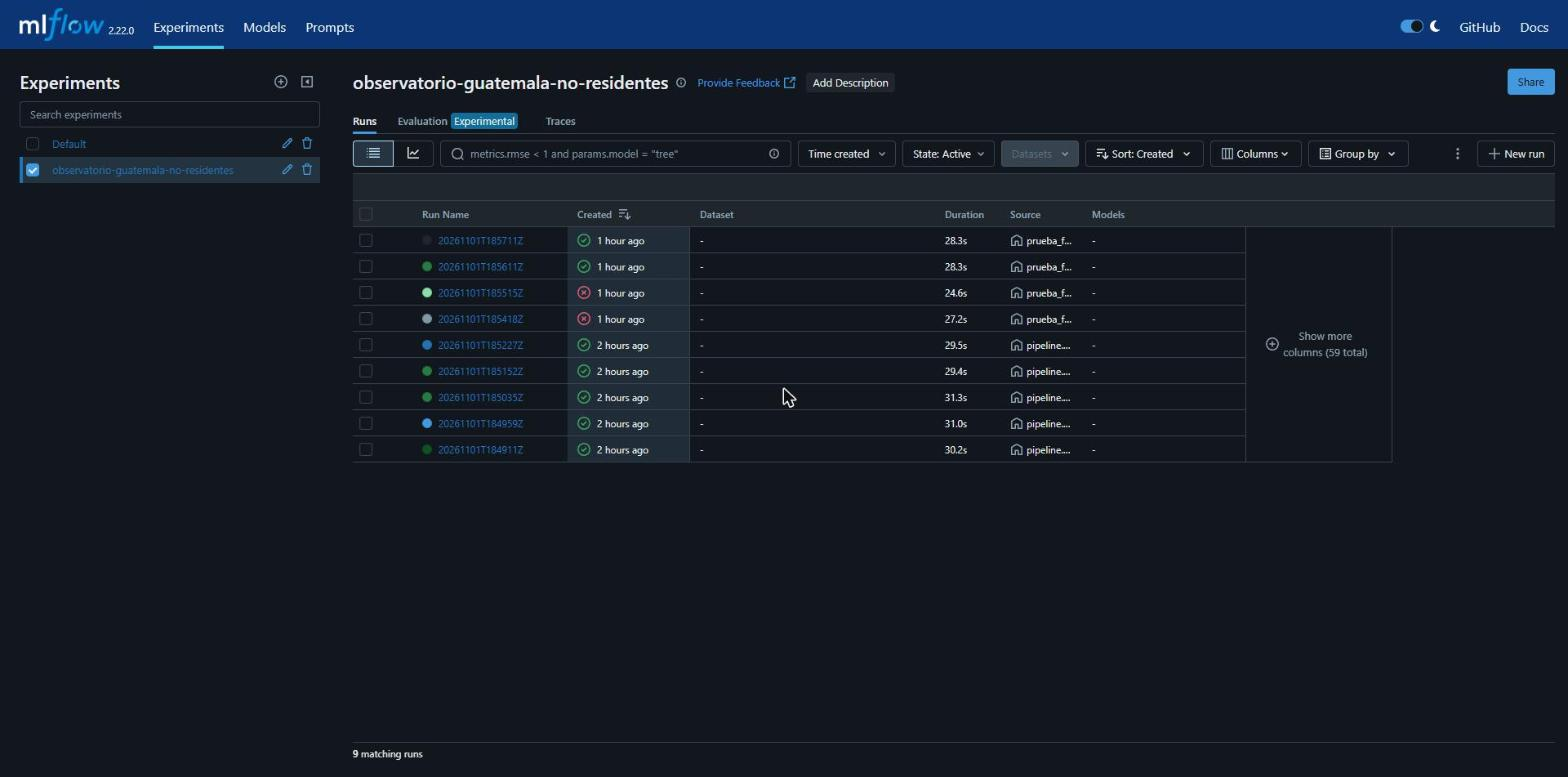
\includegraphics[width=\textwidth]{../evidencia/mlflow_ejecuciones.jpg}
\caption{Consulta de las ejecuciones en la interfaz de MLflow (\url{http://localhost:5000}), tomada después de recrear los contenedores.}
\end{figure}

%==========================================================
\section{Validación temporal y regla de aceptación}

En cada origen solo se usan los meses hasta ese origen, y los seis siguientes se estiman como si no estuvieran disponibles. El pipeline verifica que el último mes de entrenamiento sea anterior a cada mes evaluado. Una prueba automática altera un mes oculto y comprueba que su estimación no cambia. Solo se calcula el error de meses con valor observado comparable.

\textbf{Enero y febrero de 2026.} La fuente tiene esos meses observados con la misma definición, así que se evalúan dentro del origen de diciembre de 2025. Lo que no se puede reproducir es la información disponible en ese momento: solo existe la versión actual del archivo, ya revisada, y no las cifras preliminares de entonces. Además, el cambio de cobertura de cruceristas de 2023 sigue dentro de la serie. Por eso el error medido podría ser menor que el que se habría tenido en tiempo real.

\textbf{Métricas.} MAE, RMSE, WAPE (suma de errores absolutos entre suma observada) y MAPE. El MAPE excluye los meses con valor observado igual a cero e informa cuántos excluyó; en esta serie no hubo ninguno. La referencia de la regla es el ingenuo estacional. Como contexto se reportan también el último valor observado y el promedio de los 12 meses anteriores, calculados con los mismos datos y sobre los mismos meses.

\textbf{Regla} (commit \run{84d5795}, fijada antes de cualquier evaluación). Una versión candidata se aprueba solo si cumple todo lo siguiente:
\begin{enumerate}
\item Ningún control de calidad en error.
\item Salidas íntegras: columnas requeridas, los seis meses esperados, valores finitos y no negativos, \texttt{run\_id} consistente.
\item Ninguna verificación de monitoreo en error.
\item WAPE $\le$ 10\,\%. La serie promedia cerca de 295 mil visitantes por mes, así que el margen ronda 30 mil. La variación interanual habitual de un mismo mes es de 5 a 10\,\%.
\item MAE $\le 1{,}25\times$ MAE de la referencia. No se exige superarla, pero tampoco ser claramente peor que la alternativa más simple.
\end{enumerate}

\begin{figure}[H]
\centering
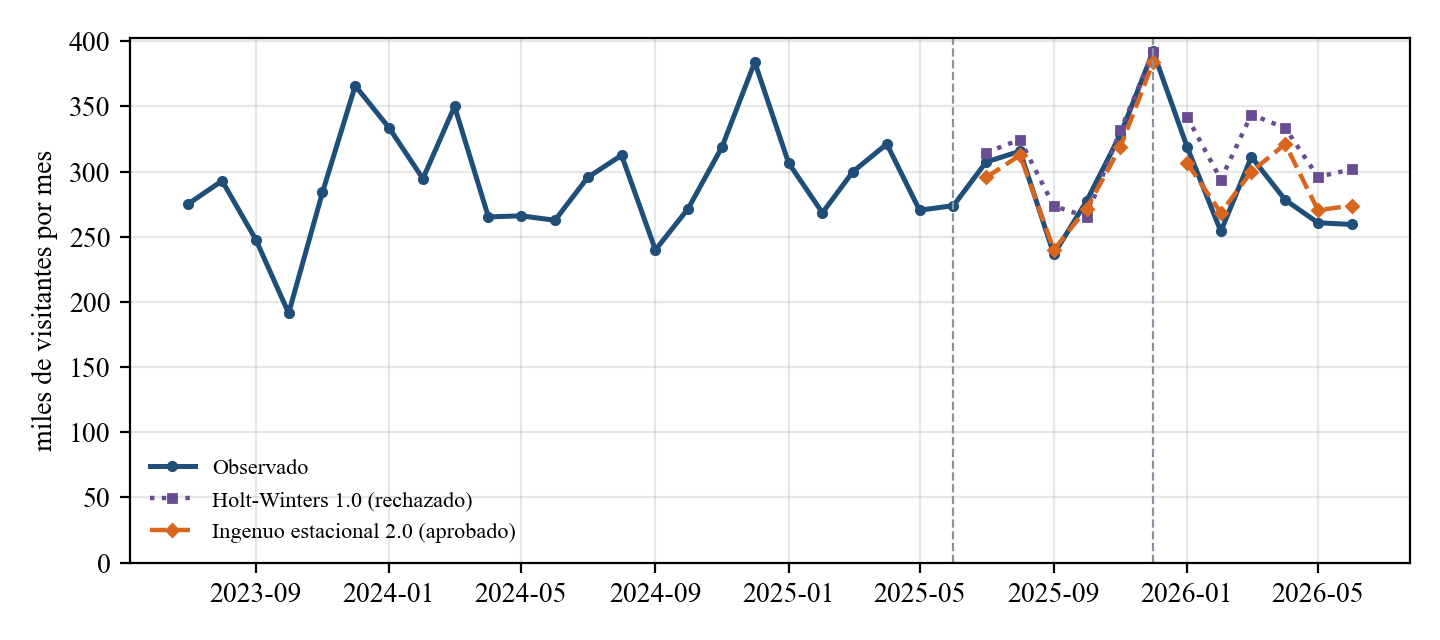
\includegraphics[width=0.95\textwidth]{validacion.png}
\caption{Validación temporal. Las líneas verticales marcan los orígenes; cada estimación usa solo datos anteriores a su origen.}
\end{figure}

\begin{table}[H]
\centering\small
\caption{Desempeño sobre los mismos 12 meses (julio 2025 -- junio 2026).}
\begin{tabular}{@{}lrrrrl@{}}
\toprule
Procedimiento & MAE & RMSE & WAPE & MAE/ref. & Decisión \\
\midrule
Holt-Winters amortiguado (v1.0, \run{f169bf4b}) & 24\,728 & 30\,126 & 8,4\,\% & 2,02 & Rechazada (criterio 5) \\
Ingenuo estacional (v2.0, \run{e528864e}) & 12\,237 & 15\,762 & 4,1\,\% & 1,00 & Aprobada \\
\midrule
Contexto: promedio de 12 meses & 34\,457 & --- & 11,7\,\% & --- & --- \\
Contexto: último valor & 79\,899 & --- & 27,1\,\% & --- & --- \\
\bottomrule
\end{tabular}
\end{table}

\textbf{Resultado.} Holt-Winters cumple el umbral de WAPE, pero su MAE duplica el de la referencia. Extrapoló la tendencia de recuperación de 2022--2024 y sobreestimó 2026 en unos 23 mil visitantes por mes (sesgo $+22{,}6$ mil). Se aplicó la regla sin modificarla y la versión 1.0 fue rechazada. La versión 2.0 retoma el procedimiento del avance del 29 de octubre, definido antes de cualquier evaluación, y se evaluó con la misma regla. Dos advertencias: el cambio de candidato se decidió después de ver los resultados (hay riesgo de selección, mitigado porque el procedimiento estaba fijado de antemano y no tiene parámetros que ajustar), y en la versión 2.0 el criterio~5 se cumple de forma trivial porque el procedimiento coincide con la referencia. Lo que de verdad decide su aprobación es el criterio~4.

%==========================================================
\section{Integración con el tablero}

La página «4 · Estimación vigente» lee \texttt{vigente.json} y la carpeta de la versión aprobada. La caché se invalida cuando cambia la fecha de modificación del puntero. Muestra la fecha de actualización, el error de validación (WAPE) explicado en lenguaje llano, los meses evaluados, el identificador de la versión y la gráfica observado/estimado (azul continuo frente a naranja con guiones y rombos, igual que en el resto del tablero). Cierra con una advertencia sobre limitaciones. Si no existe una versión aprobada, indica que las estimaciones no están disponibles. Los detalles técnicos se quedan en MLflow y en la documentación.

El archivo de estimaciones incluye \texttt{destino}, \texttt{periodo\_estimado}, \texttt{valor}, \texttt{unidad}, \texttt{tipo}, \texttt{run\_id}, \texttt{fecha\_generacion\_utc}, \texttt{version\_procedimiento} y \texttt{metodo}.

\begin{figure}[H]
\centering
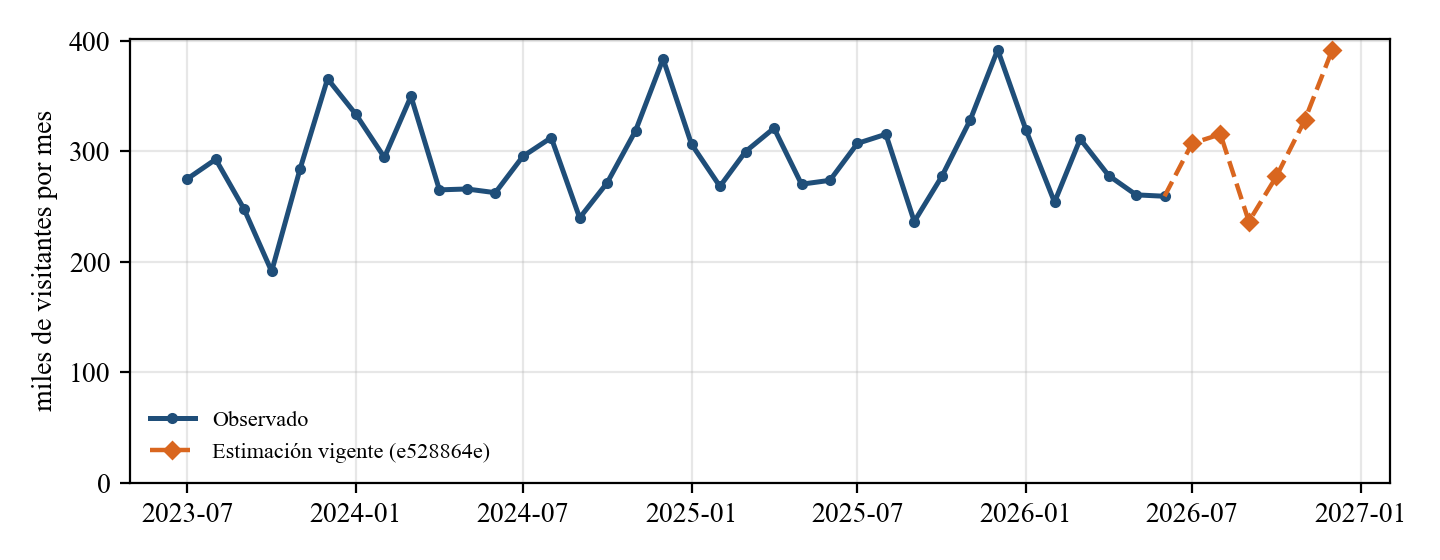
\includegraphics[width=\textwidth]{estimaciones.png}
\caption{Versión vigente: estimaciones de julio a diciembre de 2026 (entre 236 y 392 mil visitantes por mes).}
\end{figure}

%==========================================================
\section{Monitoreo y recuperación}

Cada ejecución deja \texttt{registros/<run\_id>.json} con horas de inicio y fin, etapas completadas, advertencias, errores, resultado de la publicación y versión vigente antes y después. El monitoreo hace tres verificaciones:
\begin{itemize}
\item \textbf{Actualización:} el último mes de la fuente coincide con el configurado (junio 2026) y la primera estimación es el mes siguiente.
\item \textbf{Calidad:} compara con la versión vigente el número de filas (alerta si cambia más de 10\,\%), la tasa de faltantes (más de 1 punto), los duplicados y los meses cubiertos.
\item \textbf{Resultados:} una estimación negativa o no finita es error. Una variación de más de 25\,\% frente al mismo mes del año anterior, o de más de 15\,\% frente a la versión vigente, es una alerta para revisar; por sí sola no indica pérdida de precisión. El error predictivo solo se actualiza con observaciones comparables.
\end{itemize}

La publicación es atómica: primero se escribe la carpeta temporal de la versión, después se renombra y al final se reemplaza \texttt{vigente.json}. Si una actualización falla, la versión anterior sigue disponible.

\begin{table}[H]
\centering\small
\caption{Prueba controlada (\texttt{prueba\_fallo.py}) sobre copias de la fuente; la vigente al inicio era \run{eef1c71e}.}
\begin{tabularx}{\textwidth}{@{}lYll@{}}
\toprule
Caso & Resultado & Salida & Vigente después \\
\midrule
Clave duplicada & Falla el control de unicidad; no se evalúa & 1 & \run{eef1c71e} \\
Columna \texttt{Tipo de Viajero} ausente & Falla el control de columnas y tipos & 1 & \run{eef1c71e} \\
Valores $\times1{,}4$ en jul--dic 2025 & Pasa los controles; el monitoreo alerta (+40\,\% frente a la vigente) y la regla rechaza (WAPE 20,6\,\%) & 3 & \run{eef1c71e} \\
Copia corregida (sin el duplicado) & Se publica & 0 & \run{50752886} \\
\bottomrule
\end{tabularx}
\end{table}

\textbf{Restauración.} \texttt{python lab11/restaurar.py --listar} muestra las versiones aprobadas y \texttt{python lab11/restaurar.py <run\_id>} reemplaza de forma atómica el puntero, aceptando solo versiones que cumplieron la regla. Después de la prueba se restauró \run{eef1c71e} (generada con la fuente oficial) en lugar de \run{50752886} (generada con la copia). El tablero mostró la versión restaurada sin reiniciarse, y la restauración quedó registrada en \texttt{registros/restauracion\_eef1c71e\ldots.json}. Todas las versiones aprobadas se conservan en \texttt{publicado/versiones/}.

\begin{figure}[H]
\centering
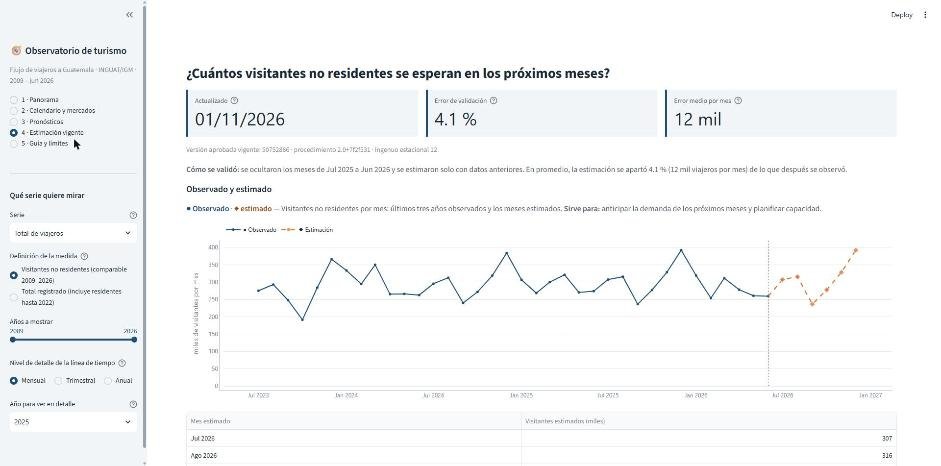
\includegraphics[width=0.82\textwidth]{../evidencia/tablero_antes_restaurar.jpg}\\[0.3em]
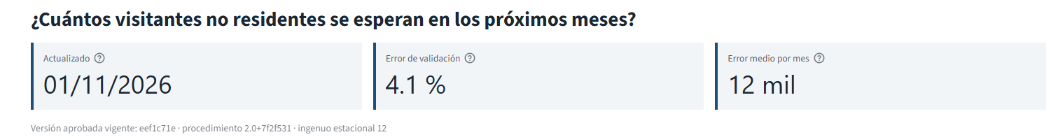
\includegraphics[width=0.82\textwidth]{../evidencia/tablero_despues_restaurar.png}
\caption{Arriba: el tablero con la versión \run{50752886}. Abajo: después de restaurar, el tablero consulta \run{eef1c71e}.}
\end{figure}

%==========================================================
\section{Docker y comprobación desde una copia limpia}

\texttt{docker-compose.yml} define tres servicios con una sola imagen: \texttt{mlflow} (puerto 5000), \texttt{tablero} (puerto 8501) y \texttt{pipeline}, que se ejecuta bajo demanda. El Excel institucional nunca entra a la imagen: \texttt{.dockerignore} es una lista blanca y la carpeta de datos se monta solo en lectura desde \texttt{LAB11\_DATOS}, que por omisión es \texttt{./Datos\_Crudos}. Los registros de MLflow y las versiones aprobadas viven en carpetas montadas del repositorio. Después de \texttt{docker compose down} no quedó ningún contenedor; al volver a levantarlos seguían las nueve ejecuciones existentes en ese momento y la misma versión vigente.

Para la copia limpia se clonó la rama en una carpeta nueva y se ejecutaron \texttt{docker compose up -d --build}, las 18 pruebas y una ejecución del pipeline. La ejecución se publicó con código sin cambios locales y con estimaciones idénticas a las vigentes, y el tablero respondió. En Windows el clon necesita \texttt{core.longpaths=true}, porque algunas rutas de artefactos superan 260 caracteres. Los pasos completos están en \texttt{lab11/README.md}.

%==========================================================
\section{Limitaciones}

\begin{itemize}
\item El ingenuo estacional no anticipa cambios de tendencia ni eventos nuevos. Su buen desempeño refleja la estabilidad de 2025--2026.
\item Doce meses evaluados son pocos para afirmar el desempeño futuro. La validación usa la versión revisada de la fuente.
\item La vía marítima perdió cobertura de cruceristas en 2023 y ese cambio sigue dentro de la serie de no residentes.
\item El cambio de candidato a la versión 2.0 se decidió después de evaluar la 1.0; lo documentan este informe, el mensaje del commit \run{78bf214} y MLflow.
\end{itemize}

\end{document}
